\documentclass{article} % For LaTeX2e
\usepackage{iclr2022_conference,times}
\usepackage{natbib}
% Optional math commands from https://github.com/goodfeli/dlbook_notation.
%%%%% NEW MATH DEFINITIONS %%%%%

\usepackage{amsmath,amsfonts,bm}

% Mark sections of captions for referring to divisions of figures
\newcommand{\figleft}{{\em (Left)}}
\newcommand{\figcenter}{{\em (Center)}}
\newcommand{\figright}{{\em (Right)}}
\newcommand{\figtop}{{\em (Top)}}
\newcommand{\figbottom}{{\em (Bottom)}}
\newcommand{\captiona}{{\em (a)}}
\newcommand{\captionb}{{\em (b)}}
\newcommand{\captionc}{{\em (c)}}
\newcommand{\captiond}{{\em (d)}}

% Highlight a newly defined term
\newcommand{\newterm}[1]{{\bf #1}}


% Figure reference, lower-case.
\def\figref#1{figure~\ref{#1}}
% Figure reference, capital. For start of sentence
\def\Figref#1{Figure~\ref{#1}}
\def\twofigref#1#2{figures \ref{#1} and \ref{#2}}
\def\quadfigref#1#2#3#4{figures \ref{#1}, \ref{#2}, \ref{#3} and \ref{#4}}
% Section reference, lower-case.
\def\secref#1{section~\ref{#1}}
% Section reference, capital.
\def\Secref#1{Section~\ref{#1}}
% Reference to two sections.
\def\twosecrefs#1#2{sections \ref{#1} and \ref{#2}}
% Reference to three sections.
\def\secrefs#1#2#3{sections \ref{#1}, \ref{#2} and \ref{#3}}
% Reference to an equation, lower-case.
\def\eqref#1{equation~\ref{#1}}
% Reference to an equation, upper case
\def\Eqref#1{Equation~\ref{#1}}
% A raw reference to an equation---avoid using if possible
\def\plaineqref#1{\ref{#1}}
% Reference to a chapter, lower-case.
\def\chapref#1{chapter~\ref{#1}}
% Reference to an equation, upper case.
\def\Chapref#1{Chapter~\ref{#1}}
% Reference to a range of chapters
\def\rangechapref#1#2{chapters\ref{#1}--\ref{#2}}
% Reference to an algorithm, lower-case.
\def\algref#1{algorithm~\ref{#1}}
% Reference to an algorithm, upper case.
\def\Algref#1{Algorithm~\ref{#1}}
\def\twoalgref#1#2{algorithms \ref{#1} and \ref{#2}}
\def\Twoalgref#1#2{Algorithms \ref{#1} and \ref{#2}}
% Reference to a part, lower case
\def\partref#1{part~\ref{#1}}
% Reference to a part, upper case
\def\Partref#1{Part~\ref{#1}}
\def\twopartref#1#2{parts \ref{#1} and \ref{#2}}

\def\ceil#1{\lceil #1 \rceil}
\def\floor#1{\lfloor #1 \rfloor}
\def\1{\bm{1}}
\newcommand{\train}{\mathcal{D}}
\newcommand{\valid}{\mathcal{D_{\mathrm{valid}}}}
\newcommand{\test}{\mathcal{D_{\mathrm{test}}}}

\def\eps{{\epsilon}}


% Random variables
\def\reta{{\textnormal{$\eta$}}}
\def\ra{{\textnormal{a}}}
\def\rb{{\textnormal{b}}}
\def\rc{{\textnormal{c}}}
\def\rd{{\textnormal{d}}}
\def\re{{\textnormal{e}}}
\def\rf{{\textnormal{f}}}
\def\rg{{\textnormal{g}}}
\def\rh{{\textnormal{h}}}
\def\ri{{\textnormal{i}}}
\def\rj{{\textnormal{j}}}
\def\rk{{\textnormal{k}}}
\def\rl{{\textnormal{l}}}
% rm is already a command, just don't name any random variables m
\def\rn{{\textnormal{n}}}
\def\ro{{\textnormal{o}}}
\def\rp{{\textnormal{p}}}
\def\rq{{\textnormal{q}}}
\def\rr{{\textnormal{r}}}
\def\rs{{\textnormal{s}}}
\def\rt{{\textnormal{t}}}
\def\ru{{\textnormal{u}}}
\def\rv{{\textnormal{v}}}
\def\rw{{\textnormal{w}}}
\def\rx{{\textnormal{x}}}
\def\ry{{\textnormal{y}}}
\def\rz{{\textnormal{z}}}

% Random vectors
\def\rvepsilon{{\mathbf{\epsilon}}}
\def\rvtheta{{\mathbf{\theta}}}
\def\rva{{\mathbf{a}}}
\def\rvb{{\mathbf{b}}}
\def\rvc{{\mathbf{c}}}
\def\rvd{{\mathbf{d}}}
\def\rve{{\mathbf{e}}}
\def\rvf{{\mathbf{f}}}
\def\rvg{{\mathbf{g}}}
\def\rvh{{\mathbf{h}}}
\def\rvu{{\mathbf{i}}}
\def\rvj{{\mathbf{j}}}
\def\rvk{{\mathbf{k}}}
\def\rvl{{\mathbf{l}}}
\def\rvm{{\mathbf{m}}}
\def\rvn{{\mathbf{n}}}
\def\rvo{{\mathbf{o}}}
\def\rvp{{\mathbf{p}}}
\def\rvq{{\mathbf{q}}}
\def\rvr{{\mathbf{r}}}
\def\rvs{{\mathbf{s}}}
\def\rvt{{\mathbf{t}}}
\def\rvu{{\mathbf{u}}}
\def\rvv{{\mathbf{v}}}
\def\rvw{{\mathbf{w}}}
\def\rvx{{\mathbf{x}}}
\def\rvy{{\mathbf{y}}}
\def\rvz{{\mathbf{z}}}

% Elements of random vectors
\def\erva{{\textnormal{a}}}
\def\ervb{{\textnormal{b}}}
\def\ervc{{\textnormal{c}}}
\def\ervd{{\textnormal{d}}}
\def\erve{{\textnormal{e}}}
\def\ervf{{\textnormal{f}}}
\def\ervg{{\textnormal{g}}}
\def\ervh{{\textnormal{h}}}
\def\ervi{{\textnormal{i}}}
\def\ervj{{\textnormal{j}}}
\def\ervk{{\textnormal{k}}}
\def\ervl{{\textnormal{l}}}
\def\ervm{{\textnormal{m}}}
\def\ervn{{\textnormal{n}}}
\def\ervo{{\textnormal{o}}}
\def\ervp{{\textnormal{p}}}
\def\ervq{{\textnormal{q}}}
\def\ervr{{\textnormal{r}}}
\def\ervs{{\textnormal{s}}}
\def\ervt{{\textnormal{t}}}
\def\ervu{{\textnormal{u}}}
\def\ervv{{\textnormal{v}}}
\def\ervw{{\textnormal{w}}}
\def\ervx{{\textnormal{x}}}
\def\ervy{{\textnormal{y}}}
\def\ervz{{\textnormal{z}}}

% Random matrices
\def\rmA{{\mathbf{A}}}
\def\rmB{{\mathbf{B}}}
\def\rmC{{\mathbf{C}}}
\def\rmD{{\mathbf{D}}}
\def\rmE{{\mathbf{E}}}
\def\rmF{{\mathbf{F}}}
\def\rmG{{\mathbf{G}}}
\def\rmH{{\mathbf{H}}}
\def\rmI{{\mathbf{I}}}
\def\rmJ{{\mathbf{J}}}
\def\rmK{{\mathbf{K}}}
\def\rmL{{\mathbf{L}}}
\def\rmM{{\mathbf{M}}}
\def\rmN{{\mathbf{N}}}
\def\rmO{{\mathbf{O}}}
\def\rmP{{\mathbf{P}}}
\def\rmQ{{\mathbf{Q}}}
\def\rmR{{\mathbf{R}}}
\def\rmS{{\mathbf{S}}}
\def\rmT{{\mathbf{T}}}
\def\rmU{{\mathbf{U}}}
\def\rmV{{\mathbf{V}}}
\def\rmW{{\mathbf{W}}}
\def\rmX{{\mathbf{X}}}
\def\rmY{{\mathbf{Y}}}
\def\rmZ{{\mathbf{Z}}}

% Elements of random matrices
\def\ermA{{\textnormal{A}}}
\def\ermB{{\textnormal{B}}}
\def\ermC{{\textnormal{C}}}
\def\ermD{{\textnormal{D}}}
\def\ermE{{\textnormal{E}}}
\def\ermF{{\textnormal{F}}}
\def\ermG{{\textnormal{G}}}
\def\ermH{{\textnormal{H}}}
\def\ermI{{\textnormal{I}}}
\def\ermJ{{\textnormal{J}}}
\def\ermK{{\textnormal{K}}}
\def\ermL{{\textnormal{L}}}
\def\ermM{{\textnormal{M}}}
\def\ermN{{\textnormal{N}}}
\def\ermO{{\textnormal{O}}}
\def\ermP{{\textnormal{P}}}
\def\ermQ{{\textnormal{Q}}}
\def\ermR{{\textnormal{R}}}
\def\ermS{{\textnormal{S}}}
\def\ermT{{\textnormal{T}}}
\def\ermU{{\textnormal{U}}}
\def\ermV{{\textnormal{V}}}
\def\ermW{{\textnormal{W}}}
\def\ermX{{\textnormal{X}}}
\def\ermY{{\textnormal{Y}}}
\def\ermZ{{\textnormal{Z}}}

% Vectors
\def\vzero{{\bm{0}}}
\def\vone{{\bm{1}}}
\def\vmu{{\bm{\mu}}}
\def\vtheta{{\bm{\theta}}}
\def\va{{\bm{a}}}
\def\vb{{\bm{b}}}
\def\vc{{\bm{c}}}
\def\vd{{\bm{d}}}
\def\ve{{\bm{e}}}
\def\vf{{\bm{f}}}
\def\vg{{\bm{g}}}
\def\vh{{\bm{h}}}
\def\vi{{\bm{i}}}
\def\vj{{\bm{j}}}
\def\vk{{\bm{k}}}
\def\vl{{\bm{l}}}
\def\vm{{\bm{m}}}
\def\vn{{\bm{n}}}
\def\vo{{\bm{o}}}
\def\vp{{\bm{p}}}
\def\vq{{\bm{q}}}
\def\vr{{\bm{r}}}
\def\vs{{\bm{s}}}
\def\vt{{\bm{t}}}
\def\vu{{\bm{u}}}
\def\vv{{\bm{v}}}
\def\vw{{\bm{w}}}
\def\vx{{\bm{x}}}
\def\vy{{\bm{y}}}
\def\vz{{\bm{z}}}

% Elements of vectors
\def\evalpha{{\alpha}}
\def\evbeta{{\beta}}
\def\evepsilon{{\epsilon}}
\def\evlambda{{\lambda}}
\def\evomega{{\omega}}
\def\evmu{{\mu}}
\def\evpsi{{\psi}}
\def\evsigma{{\sigma}}
\def\evtheta{{\theta}}
\def\eva{{a}}
\def\evb{{b}}
\def\evc{{c}}
\def\evd{{d}}
\def\eve{{e}}
\def\evf{{f}}
\def\evg{{g}}
\def\evh{{h}}
\def\evi{{i}}
\def\evj{{j}}
\def\evk{{k}}
\def\evl{{l}}
\def\evm{{m}}
\def\evn{{n}}
\def\evo{{o}}
\def\evp{{p}}
\def\evq{{q}}
\def\evr{{r}}
\def\evs{{s}}
\def\evt{{t}}
\def\evu{{u}}
\def\evv{{v}}
\def\evw{{w}}
\def\evx{{x}}
\def\evy{{y}}
\def\evz{{z}}

% Matrix
\def\mA{{\bm{A}}}
\def\mB{{\bm{B}}}
\def\mC{{\bm{C}}}
\def\mD{{\bm{D}}}
\def\mE{{\bm{E}}}
\def\mF{{\bm{F}}}
\def\mG{{\bm{G}}}
\def\mH{{\bm{H}}}
\def\mI{{\bm{I}}}
\def\mJ{{\bm{J}}}
\def\mK{{\bm{K}}}
\def\mL{{\bm{L}}}
\def\mM{{\bm{M}}}
\def\mN{{\bm{N}}}
\def\mO{{\bm{O}}}
\def\mP{{\bm{P}}}
\def\mQ{{\bm{Q}}}
\def\mR{{\bm{R}}}
\def\mS{{\bm{S}}}
\def\mT{{\bm{T}}}
\def\mU{{\bm{U}}}
\def\mV{{\bm{V}}}
\def\mW{{\bm{W}}}
\def\mX{{\bm{X}}}
\def\mY{{\bm{Y}}}
\def\mZ{{\bm{Z}}}
\def\mBeta{{\bm{\beta}}}
\def\mPhi{{\bm{\Phi}}}
\def\mLambda{{\bm{\Lambda}}}
\def\mSigma{{\bm{\Sigma}}}

% Tensor
\DeclareMathAlphabet{\mathsfit}{\encodingdefault}{\sfdefault}{m}{sl}
\SetMathAlphabet{\mathsfit}{bold}{\encodingdefault}{\sfdefault}{bx}{n}
\newcommand{\tens}[1]{\bm{\mathsfit{#1}}}
\def\tA{{\tens{A}}}
\def\tB{{\tens{B}}}
\def\tC{{\tens{C}}}
\def\tD{{\tens{D}}}
\def\tE{{\tens{E}}}
\def\tF{{\tens{F}}}
\def\tG{{\tens{G}}}
\def\tH{{\tens{H}}}
\def\tI{{\tens{I}}}
\def\tJ{{\tens{J}}}
\def\tK{{\tens{K}}}
\def\tL{{\tens{L}}}
\def\tM{{\tens{M}}}
\def\tN{{\tens{N}}}
\def\tO{{\tens{O}}}
\def\tP{{\tens{P}}}
\def\tQ{{\tens{Q}}}
\def\tR{{\tens{R}}}
\def\tS{{\tens{S}}}
\def\tT{{\tens{T}}}
\def\tU{{\tens{U}}}
\def\tV{{\tens{V}}}
\def\tW{{\tens{W}}}
\def\tX{{\tens{X}}}
\def\tY{{\tens{Y}}}
\def\tZ{{\tens{Z}}}


% Graph
\def\gA{{\mathcal{A}}}
\def\gB{{\mathcal{B}}}
\def\gC{{\mathcal{C}}}
\def\gD{{\mathcal{D}}}
\def\gE{{\mathcal{E}}}
\def\gF{{\mathcal{F}}}
\def\gG{{\mathcal{G}}}
\def\gH{{\mathcal{H}}}
\def\gI{{\mathcal{I}}}
\def\gJ{{\mathcal{J}}}
\def\gK{{\mathcal{K}}}
\def\gL{{\mathcal{L}}}
\def\gM{{\mathcal{M}}}
\def\gN{{\mathcal{N}}}
\def\gO{{\mathcal{O}}}
\def\gP{{\mathcal{P}}}
\def\gQ{{\mathcal{Q}}}
\def\gR{{\mathcal{R}}}
\def\gS{{\mathcal{S}}}
\def\gT{{\mathcal{T}}}
\def\gU{{\mathcal{U}}}
\def\gV{{\mathcal{V}}}
\def\gW{{\mathcal{W}}}
\def\gX{{\mathcal{X}}}
\def\gY{{\mathcal{Y}}}
\def\gZ{{\mathcal{Z}}}

% Sets
\def\sA{{\mathbb{A}}}
\def\sB{{\mathbb{B}}}
\def\sC{{\mathbb{C}}}
\def\sD{{\mathbb{D}}}
% Don't use a set called E, because this would be the same as our symbol
% for expectation.
\def\sF{{\mathbb{F}}}
\def\sG{{\mathbb{G}}}
\def\sH{{\mathbb{H}}}
\def\sI{{\mathbb{I}}}
\def\sJ{{\mathbb{J}}}
\def\sK{{\mathbb{K}}}
\def\sL{{\mathbb{L}}}
\def\sM{{\mathbb{M}}}
\def\sN{{\mathbb{N}}}
\def\sO{{\mathbb{O}}}
\def\sP{{\mathbb{P}}}
\def\sQ{{\mathbb{Q}}}
\def\sR{{\mathbb{R}}}
\def\sS{{\mathbb{S}}}
\def\sT{{\mathbb{T}}}
\def\sU{{\mathbb{U}}}
\def\sV{{\mathbb{V}}}
\def\sW{{\mathbb{W}}}
\def\sX{{\mathbb{X}}}
\def\sY{{\mathbb{Y}}}
\def\sZ{{\mathbb{Z}}}

% Entries of a matrix
\def\emLambda{{\Lambda}}
\def\emA{{A}}
\def\emB{{B}}
\def\emC{{C}}
\def\emD{{D}}
\def\emE{{E}}
\def\emF{{F}}
\def\emG{{G}}
\def\emH{{H}}
\def\emI{{I}}
\def\emJ{{J}}
\def\emK{{K}}
\def\emL{{L}}
\def\emM{{M}}
\def\emN{{N}}
\def\emO{{O}}
\def\emP{{P}}
\def\emQ{{Q}}
\def\emR{{R}}
\def\emS{{S}}
\def\emT{{T}}
\def\emU{{U}}
\def\emV{{V}}
\def\emW{{W}}
\def\emX{{X}}
\def\emY{{Y}}
\def\emZ{{Z}}
\def\emSigma{{\Sigma}}

% entries of a tensor
% Same font as tensor, without \bm wrapper
\newcommand{\etens}[1]{\mathsfit{#1}}
\def\etLambda{{\etens{\Lambda}}}
\def\etA{{\etens{A}}}
\def\etB{{\etens{B}}}
\def\etC{{\etens{C}}}
\def\etD{{\etens{D}}}
\def\etE{{\etens{E}}}
\def\etF{{\etens{F}}}
\def\etG{{\etens{G}}}
\def\etH{{\etens{H}}}
\def\etI{{\etens{I}}}
\def\etJ{{\etens{J}}}
\def\etK{{\etens{K}}}
\def\etL{{\etens{L}}}
\def\etM{{\etens{M}}}
\def\etN{{\etens{N}}}
\def\etO{{\etens{O}}}
\def\etP{{\etens{P}}}
\def\etQ{{\etens{Q}}}
\def\etR{{\etens{R}}}
\def\etS{{\etens{S}}}
\def\etT{{\etens{T}}}
\def\etU{{\etens{U}}}
\def\etV{{\etens{V}}}
\def\etW{{\etens{W}}}
\def\etX{{\etens{X}}}
\def\etY{{\etens{Y}}}
\def\etZ{{\etens{Z}}}

% The true underlying data generating distribution
\newcommand{\pdata}{p_{\rm{data}}}
% The empirical distribution defined by the training set
\newcommand{\ptrain}{\hat{p}_{\rm{data}}}
\newcommand{\Ptrain}{\hat{P}_{\rm{data}}}
% The model distribution
\newcommand{\pmodel}{p_{\rm{model}}}
\newcommand{\Pmodel}{P_{\rm{model}}}
\newcommand{\ptildemodel}{\tilde{p}_{\rm{model}}}
% Stochastic autoencoder distributions
\newcommand{\pencode}{p_{\rm{encoder}}}
\newcommand{\pdecode}{p_{\rm{decoder}}}
\newcommand{\precons}{p_{\rm{reconstruct}}}

\newcommand{\laplace}{\mathrm{Laplace}} % Laplace distribution

\newcommand{\E}{\mathbb{E}}
\newcommand{\Ls}{\mathcal{L}}
\newcommand{\R}{\mathbb{R}}
\newcommand{\emp}{\tilde{p}}
\newcommand{\lr}{\alpha}
\newcommand{\reg}{\lambda}
\newcommand{\rect}{\mathrm{rectifier}}
\newcommand{\softmax}{\mathrm{softmax}}
\newcommand{\sigmoid}{\sigma}
\newcommand{\softplus}{\zeta}
\newcommand{\KL}{D_{\mathrm{KL}}}
\newcommand{\Var}{\mathrm{Var}}
\newcommand{\standarderror}{\mathrm{SE}}
\newcommand{\Cov}{\mathrm{Cov}}
% Wolfram Mathworld says $L^2$ is for function spaces and $\ell^2$ is for vectors
% But then they seem to use $L^2$ for vectors throughout the site, and so does
% wikipedia.
\newcommand{\normlzero}{L^0}
\newcommand{\normlone}{L^1}
\newcommand{\normltwo}{L^2}
\newcommand{\normlp}{L^p}
\newcommand{\normmax}{L^\infty}

\newcommand{\parents}{Pa} % See usage in notation.tex. Chosen to match Daphne's book.

\DeclareMathOperator*{\argmax}{arg\,max}
\DeclareMathOperator*{\argmin}{arg\,min}

\DeclareMathOperator{\sign}{sign}
\DeclareMathOperator{\Tr}{Tr}
\let\ab\allowbreak


%######## APS360: Uncomment your submission name
%\newcommand{\apsname}{Project Proposal}
%\newcommand{\apsname}{Progress Report}
\newcommand{\apsname}{Final Report}

%######## APS360: Put your Group Number here
\newcommand{\gpnumber}{33}

\usepackage{hyperref}
\usepackage{url}
\usepackage{graphicx}
\usepackage{booktabs}
\usepackage{multirow}
\usepackage{tabularx}
\usepackage{float}

%######## APS360: Put your project Title here
\title{Skin Disease Detection Using Deep Learning}

%######## APS360: Put your names, student IDs and Emails here
\author{Jacky Li  \\
Student\# 1011271678\\
\texttt{jakkii.li@mail.utoronto.ca} \\
\And
Jordan Cui  \\
Student\# 1011026916 \\
\texttt{jordan.cui@mail.utoronto.ca \phantom{    }} \\
\AND
Lawrence Ding  \\
Student\# 1011439025 \\
\texttt{larryzm.ding@mail.utoronto.ca} \\
\And
Soham Shorey \\
Student\# 1010845169 \\
\texttt{soham.shorey@mail.utoronto.ca} \\
\AND
}

\newcommand{\fix}{\marginpar{FIX}}
\newcommand{\new}{\marginpar{NEW}}

\iclrfinalcopy 
%######## APS360: Document starts here
\begin{document}

\maketitle

\vspace{-1cm}

\begin{abstract}
This project presents a deep-learning based approach for multi-class classification of dermatological conditions, including melanoma, actinic keratosis, and seven other forms of benign and malignant lesions by analyzing skin images. Early and accurate detection of skin diseases can significantly improve patient outcomes, particularly for malignant conditions such as melanoma. A combined dataset of 24,738 images from four public sources (BCN20000 \citep{isic_bcn20000}, HAM10000 \citep{ham10000_dataset}, PAD-UFES-20 \citep{pad_ufes_dataset}, and DERM12345 \citep{yilmaz2024derm12345}) was constructed. Labels were standardized through preprocessing, classes were balanced through undersampling and data augmentation, and all images were resized to $512 \times 512$.

The best-performing model uses a pretrained Swin Transformer Base backbone followed by a two-layer fully connected classifier. Class imbalance was addressed with a combination of oversampling, WeightedRandomSampler, Mixup/CutMix augmentations, and Class-Balanced Focal Loss with medical importance weighting. A baseline model using ResNet18 feature extraction and KNN classifier achieved 56.3\% accuracy.

The proposed model achieved 89.1\% test accuracy, 91.3\% precision, 88.5\% recall, and 89.8\% macro F1-score, substantially outperforming the baseline. These results demonstrate the potential of transformer-based architectures as a supportive diagnostic tool. Future work includes further improving minority class performance, incorporating additional data sources, and validating the model on external datasets to assess clinical applicability.
%######## APS360: Do not change the next line. This shows your Main body page count.
----Total Pages: \pageref{last_page}
\end{abstract}

\section{Introduction}

This report outlines a deep learning model to classify dermatological conditions, including melanoma, keratosis, basal cell carcinoma, and actinic keratosis from skin images. This model allows patients to detect dangerous skin conditions like melanoma early and assists healthcare professionals in their diagnosis.

Skin conditions are among the most widespread and varied health conditions, affecting over one-third of the global population \citep{li2024epidemiological}. In Canada, the incidence of skin conditions like melanoma has increased by more than 2\% annually since the 1980s \citep{canadian_dermatology_association}. This rise strains healthcare systems worldwide. In 2013 alone, 84 million Americans sought medical attention for a skin-related issue \citep{american_academy_dermatology}. Our skin classifier could alleviate this burden on healthcare infrastructure by encouraging patients to seek medical attention before their condition deteriorates and by assisting in diagnosis.

Deep learning models, such as convolutional neural networks (CNNs) and vision transformers (ViTs), are highly effective for skin disease classification from images because of their ability to extract spatial patterns. CNN-based and transformer skin disease classifiers have already been implemented (see Section 3) with promising results for physicians and patients.

\section{Illustration/Figure}

\begin{figure}[H]
\begin{center}
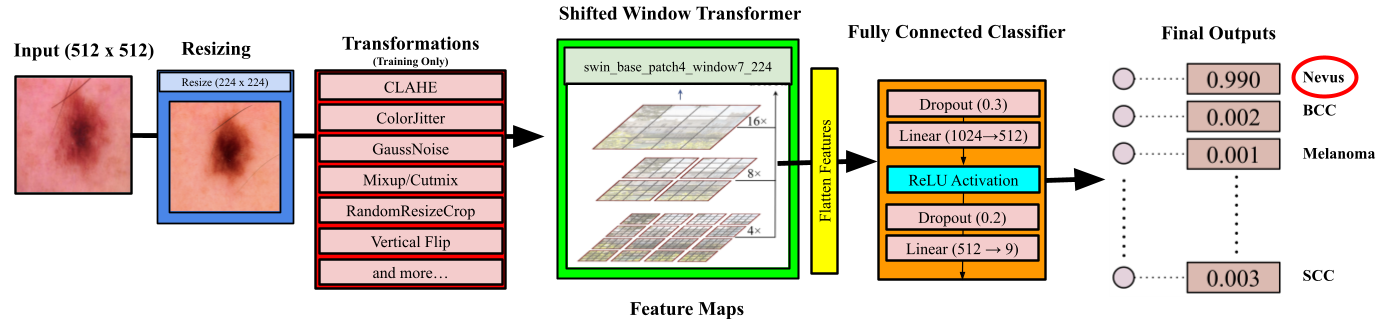
\includegraphics[width=1\textwidth]{Figs/swin_architecture.png}
\end{center}
\caption{Overview of our model architecture using a Swin Transformer. The model processes image patches through shifted window attention mechanisms for hierarchical feature learning.}
\label{fig:swin_architecture}
\end{figure}

\section{Background/Related Work}

Machine learning models for skin disease detection have been widely studied and are now available to consumers through websites and mobile applications.

Several studies focus on detecting skin cancer from images. For example, a 2017 study compared the performance of two convolutional neural network (CNN) models trained on over 120,000 images to distinguish between keratinocyte carcinomas and benign seborrheic keratoses, as well as malignant melanomas and benign nevi with the diagnostic accuracy of 21 board-certified dermatologists \citep{esteva2017dermatologist}. Unlike earlier models limited to standardized dermoscopy and histology images, this model was trained to handle dermoscopy and smartphone-quality images, improving usability for everyday users.

Another study used the Microsoft ResNet-152 CNN model, trained on 19,398 images, to assess the probability of 12 distinct skin conditions and to differentiate between benign and malignant cases. The model achieved AUC scores ranging from 0.82 to 0.96, comparable to healthcare professionals \citep{han2018classification}. Variations of ResNet have been implemented frequently in studies. For example, a 2025 study uses a self-reliant residual network (SR-ResNet) to identify melanoma \citep{radhika2025self}. It uses Zoutendijk's Method, a nonlinear optimizer that selects optimal step size and direction to stabilize convergence and prevent gradient vanishing and overfitting. The model achieved an accuracy of 94.79\%, precision of 93.09\%, and recall of 96.62\%, outperforming traditional deep learning models.

Beyond skin cancer, studies have used models to classify a wider range of skin diseases. For instance, a 2019 study evaluated five different models for classifying three types of skin diseases, with CNNs achieving high 90s precision and recall scores \citep{bhadula2019machine}. These studies underscore the utility of machine learning, particularly CNNs, in skin disease detection.

Machine learning models that detect skin conditions are readily available on websites and mobile applications. DermascanAI uses an EfficientNetB0-based network, predicting nine common skin conditions with 87.2\% accuracy \citep{vadivelraju2025dermascan}. SkinVision detected premalignant and malignant skin lesions with 86.9\% sensitivity and 70.4\% specificity \citep{sangers2022validation}.

These studies and existing successful models helped inform our choices of model architecture.

\section{Data Processing}

We combined and preprocessed four public skin lesion datasets to create a dataset that covers various skin conditions, skin types, and imaging methods.

\subsection{Data Sources}

Our data was sourced from four datasets: BCN20000 \citep{isic_bcn20000}, HAM10000 \citep{ham10000_dataset}, PAD-UFES-20 \citep{pad_ufes_dataset}, and DERM12345 \citep{yilmaz2024derm12345}.

\begin{table}[H]
\caption{Statistics on Data Sources. Datasets contain different image sizes, class counts, and formats.}
\label{data-sources}
\begin{center}
\footnotesize
\begin{tabularx}{\textwidth}{|l|p{1cm}|c|c|X|X|}
\hline
\textbf{Dataset} & \textbf{Classes} & \textbf{Images} & \textbf{Size} & \textbf{Format/Extraction Process} & \textbf{Source(s)} \\
\hline
BCN20000 & 8 & 18946 & $256 \times 256$ & Extracted BCN20000 images from ISIC archive using metadata CSV file & ISIC archive \\
\hline
HAM10000 & 7 & 10015 & $450 \times 600$ & Downloaded from Kaggle and stored in 2 separate folders which were combined & Medical University of Vienna, Austria, \& the skin cancer practice of Cliff Rosendahl in Queensland \\
\hline
PAD-UFES-20 & 6 & 2298 & Varies & Downloaded from Kaggle and stored in 3 folders which were combined & Federal University of Espírito Santo (UFES) in Brazil \\
\hline
DERM12345 & 40 (subclasses) & 12345 & $256 \times 256$ & Extracted DERM12345 images from ISIC archive using CSV file & ISIC archive \\
\hline
\end{tabularx}
\end{center}
\end{table}

\subsection{Data Cleaning \& Preprocessing}

The unification of these four datasets required several preprocessing steps.

The BCN20000 \citep{isic_bcn20000} and DERM12345 \citep{yilmaz2024derm12345} datasets were not publicly separated from the broader ISIC archive, so we used their respective CSV files to isolate and download their labelled images. The HAM10000 \citep{ham10000_dataset} and PAD-UFES-20 \citep{pad_ufes_dataset} datasets were downloaded from Kaggle, with their respective folders being organized into unified directories.

Data labels were extracted from the diagnosis\_3 field in BCN2000 and DERM12345, the dx field in HAM10000, and the diagnostic field in the PAD-UFES-20 CSV. We standardized all labels into nine unified classes: nevus, melanoma, actinic (precancerous) keratosis, basal cell carcinoma (BCC), squamous cell carcinoma (SCC), lentigo, vascular lesion, dermatofibroma, and (benign) keratosis. The images labelled under each class were placed into corresponding folders using a label mapping system. Nevus images were undersampled to prevent severe dataset imbalance and other labels were ignored. Table~\ref{dataset-size} shows the size of our dataset after preprocessing.


\begin{table}[H]
\caption{Dataset size after preprocessing.}
\label{dataset-size}
\begin{center}
\footnotesize
\begin{tabular}{lccccc}
\toprule
\textbf{Class} & \textbf{Nevus} & \textbf{Melanoma} & \textbf{BCC} & \textbf{Keratosis} & \textbf{Actinic Keratosis} \\
\textbf{Count} & 7500 & 6149 & 4613 & 2982 & 1473 \\
\midrule
\textbf{Class} & \textbf{SCC} & \textbf{Dermatofibroma} & \textbf{Lentigo} & \textbf{Vascula Lesions} & \\
\textbf{Count} & 862 & 463 & 374 & 322 & \\
\midrule
\multicolumn{6}{c}{\textbf{Total: 24738}} \\
\bottomrule
\end{tabular}
\end{center}
\end{table}

Before consolidation, we also resized all images to $512 \times 512$ using the PIL.Image library for image size flexibility in different models. For instance, our final model inputs $224 \times 224$ images.

The final dataset contains 9 classes of $512 \times 512$ images in different formats, including dermatoscopic imaging and phone photos, ensuring the robustness of our model to different types of data.


\begin{figure}[H]
\begin{center}
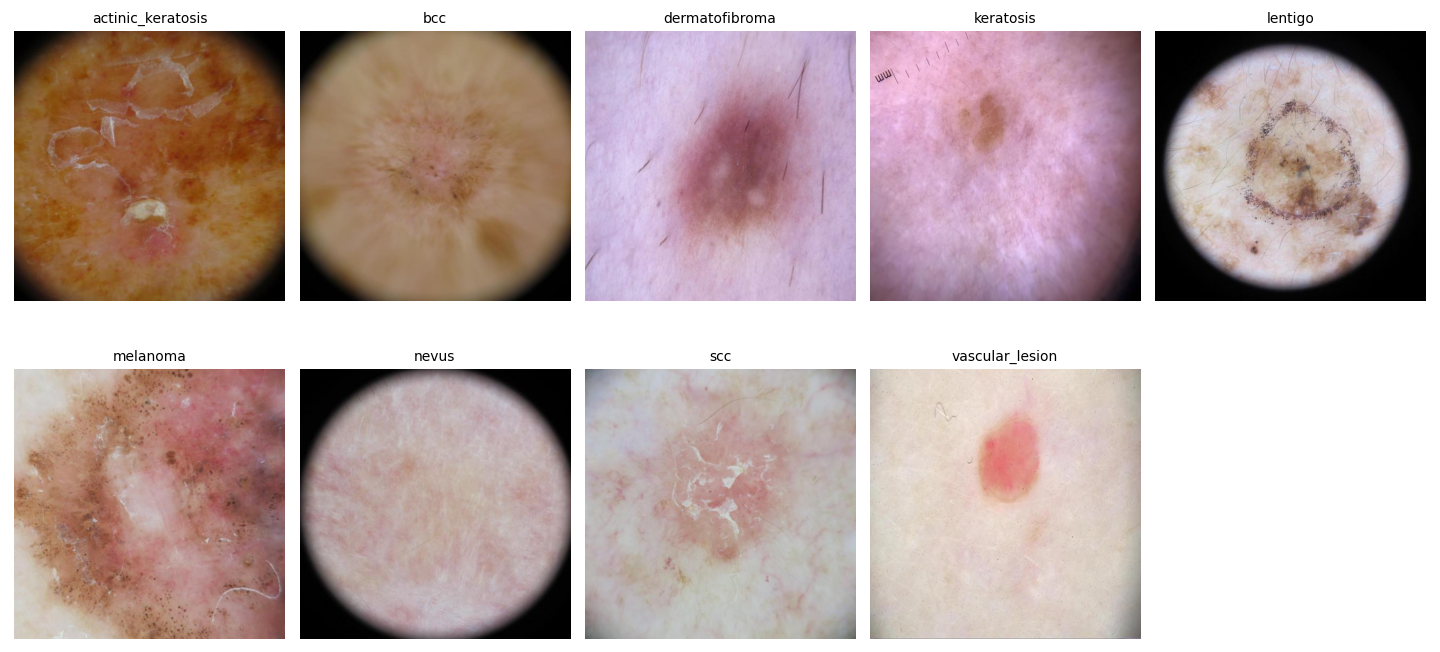
\includegraphics[width=0.8\textwidth]{Figs/sample_images.png}
\end{center}
\caption{Sample resized and labelled images from each of the 9 classes in the combined dataset.}
\label{fig:sample_images}
\end{figure}


We split the processed dataset into 70\% training, 15\% validation, and 15\% test sets to ensure robust model training and evaluation. Each split maintains the same class distribution as visualized in Figure~\ref{fig:class_distribution}. However, the dataset remains imbalanced, with the \textit{nevus} and \textit{melanoma} classes accounting for 55\% of the data.


\begin{figure}[H]
\begin{center}
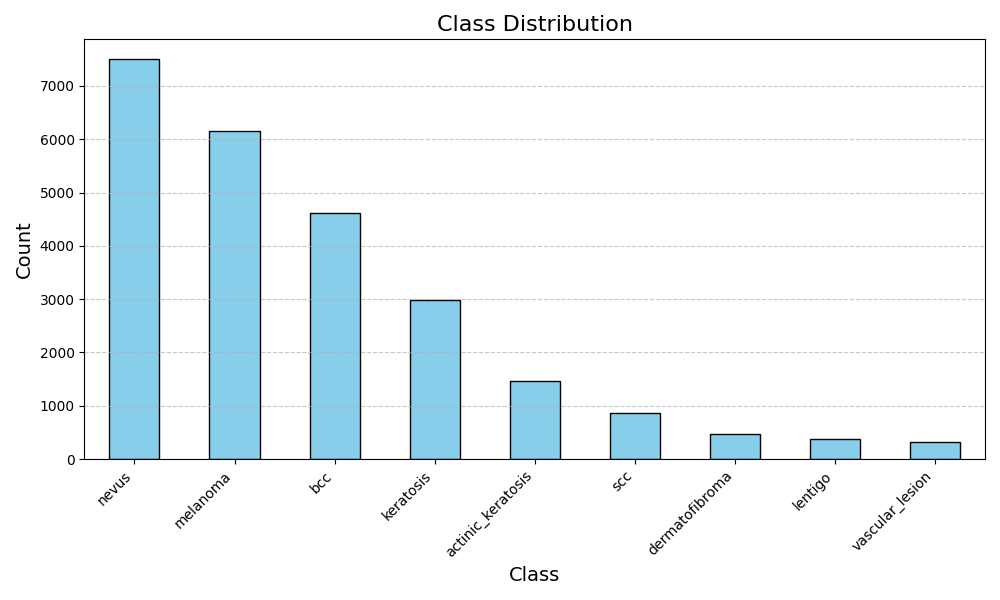
\includegraphics[width=0.6\textwidth]{Figs/class_distribution.png}
\end{center}
\caption{Class Distribution of Combined Dataset}
\label{fig:class_distribution}
\end{figure}



\section{Architecture}

An illustration of the model architecture is shown in Figure \ref{fig:swin_architecture}.

\subsection{Model Architecture}

Our best model uses the Swin Transformer Base backbone (swin\_base\_patch4\_window7\_224) pretrained on ImageNet. A vision transformer model was chosen due to its higher modeling capacity and lower inductive biases than CNNs. This specific vision transformer processes 4x4 non-overlapping image patches through multi-head self-attention within 7x7 shifted windows. These patches are merged to form multi-scale feature maps. The Swin backbones' pooled feature vector is passed to a 2-layer fully connected linear classifier head with ReLU activation and dropout layers to prevent overfitting. The hidden layer has 512 units and the final layer has 9 units for the 9 skin disease classes. The combined model is extremely large compared to CNN counterparts, with almost 90 million parameters.

\subsection{Training Techniques}
\label{subsec:training_techniques}

This class imbalance was addressed using various data sampling and augmentation techniques. During training, we applied 29 different image transformations, including ColorJitter, RandomResizedCrop, Vertical Flip and CLAHE (a dermatology focused contrast normalization) with more transformations applied to minority and challenging classes. Additionally, we used WeightedRandomSampler and oversampling of minority classes to balance the classes seen in training and Mixup/CutMix for 80\% of the training epochs which blend both images and labels together to improve performance metrics and smooth decision boundaries. These techniques boosted the model's metrics and robustness by addressing the class imbalance.

During the Mixup/CutMix epochs, the model uses soft-target cross-entropy loss, which directly compares the predicted probability distribution to the soft labels from the augmentation (alpha\_mixup = 0.3, alpha\_cutmix = 1.0, label\_smoothing =0.1). After 80\% of epochs are completed, the model uses Class-Balanced Focal Loss ($\gamma$ = 2.0) to reward classifying difficult samples. The class weights inside this loss are computed from the effective number of samples formula ($\beta$ = 0.9999) and are further scaled by medical importance factors, which give higher priority to more dangerous conditions shown in Table~\ref{medical-importance}.

The model was trained for 200 epochs with a batch size of 16 using the AdamW optimizer with a learning rate of 1e-4, weight decay of 1e-4, betas of 0.9 and 0.999. The learning rate schedule combined 3 stages: a linear warmup for the first 5\% of epochs, followed by cosine annealing with warm restarts (restart period $\approx$ 12.5\% of remaining epochs, ReduceLROnPlateau stage triggered by stagnation in macro F1 over 8 epochs. Early stopping was applied if macro F1 did not improve for 35 epochs.

\begin{table}[H]
\caption{Medical Importance Factors per Class}
\label{medical-importance}
\begin{center}
\footnotesize
\begin{tabularx}{\textwidth}{|l|c|X|}
\hline
\textbf{Class Name} & \textbf{Medical Importance Weight} & \textbf{Notes} \\
\hline
nevus & 1.0 & Most common, baseline weight \\
\hline
melanoma & 3.0 & Life-threatening malignancy \\
\hline
bcc & 2.0 & Malignant but less aggressive \\
\hline
keratosis & 2.2 & Challenging to distinguish from actinic keratosis \\
\hline
actinic\_keratosis & 2.5 & Pre-cancerous lesion \\
\hline
scc & 2.5 & Malignant, clinically important \\
\hline
dermatofibroma & 1.8 & Benign, important for differential diagnosis \\
\hline
lentigo & 2.3 & Age-related, challenging morphology \\
\hline
vascular\_lesion & 1.8 & Specific diagnosis, moderate importance \\
\hline
\end{tabularx}
\end{center}
\end{table}

\section{Baseline Model}

For the baseline model, a hybrid approach combining pre-trained feature extraction with a simple classifier was selected. Direct use of simple algorithms such as support vector machines (SVM) or k-nearest neighbors (KNN) on raw images was deemed unsuitable as a baseline due to the complexity of skin disease classification and the high-dimensional nature of image data, which would likely result in near-chance performance. Instead, a pre-trained ResNet18 model was employed for feature extraction. All input images were rescaled from 512 × 512 to 224 × 224 pixels to match the ResNet18 input requirements. The model's fully connected layers were removed, retaining only the convolutional and average pooling layers, which output a fixed-length feature vector for each image. These feature vectors were then used as input to a KNN classifier implemented in scikit-learn with the n\_neighbors parameter set to 8. This baseline achieved a test accuracy of 56.32\%, surpassing the random-chance baseline of 11.11\%. Although the resulting F1-scores indicate limited suitability for real-world application, the approach provides a reproducible and reasonable benchmark for evaluating the performance of more complex neural network architectures.

\begin{figure}[H]
\begin{center}
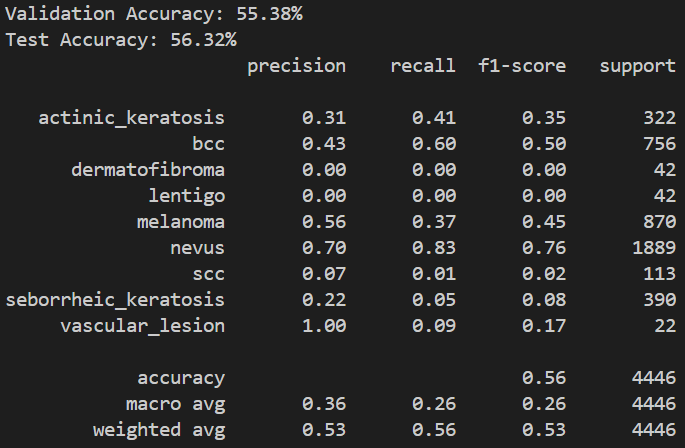
\includegraphics[width=0.5\textwidth]{Figs/baseline_results.png}
\end{center}
\caption{Baseline model performance metrics. This model struggles with the imbalanced dataset, with higher F1-scores for the more common classes, but extremely low for the less common classes.}
\end{figure}

\section{Quantitative and Qualitative Results}

\subsection{Quantitative Results}

Our final Swin Transformer Base skin detection model achieved a best validation accuracy of 90.2\%, F1 of 88.0\%, precision of 92.0\% and recall of 85.4\% on the 9 classes. Training metrics and losses are not directly comparable to validation results due to the use of a WeightedRandomSampler and extensive data augmentation, which altered the training distribution.

\begin{figure}[H]
\begin{center}
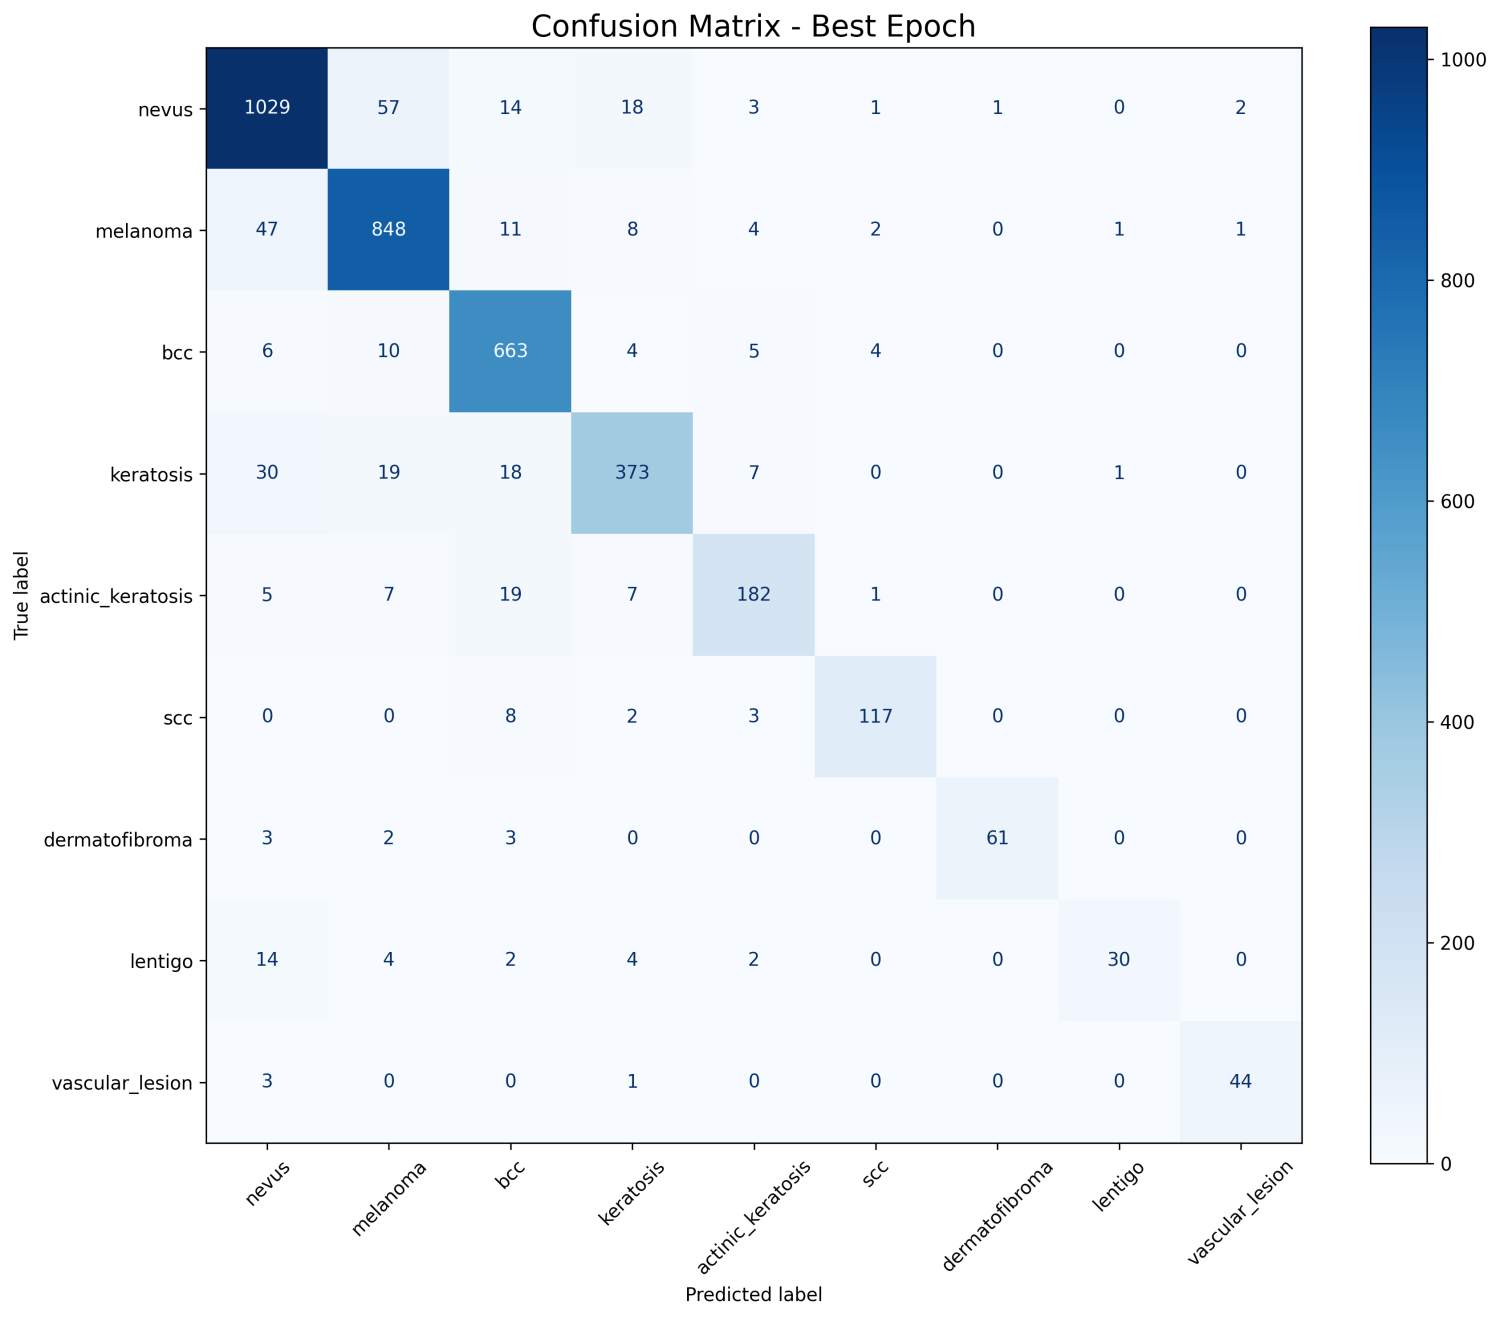
\includegraphics[width=0.7\textwidth]{Figs/confusion_matrix.png}
\end{center}
\caption{Confusion matrix of our best model checkpoint evaluated on the validation data set.}
\end{figure}

The final model was trained over 170 epochs with frequent checkpoints. Additional augmentations and loss function adjustments were introduced around the 60th epoch, causing the training loss spikes seen in Figure~\ref{fig:training_metrics} but improving validation performance. The loss function started as soft cross-entropy with heavy augmentation for 80\% of epochs, then switched to class-balanced focal loss with reduced augmentation for convergence.


\begin{figure}[H]
\begin{center}
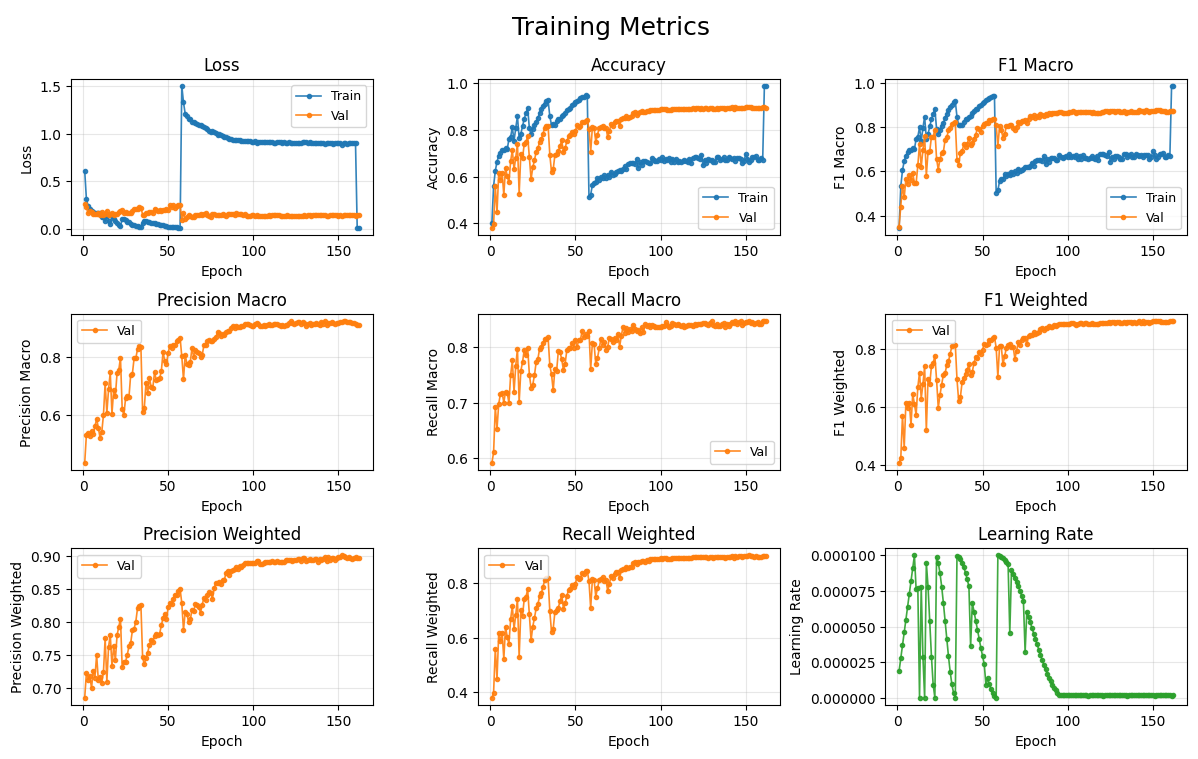
\includegraphics[width=0.6\textwidth]{Figs/training_metrics.png}
\end{center}
\caption{Training Metrics. From the top left graphs show loss, accuracy, macro F1, macro precision, macro recall, weighted f1, weighted precision, weighted recall, and learning rate. Horizontal axis shows epochs, with a total of 170. Blue represents train set while orange represents validation.}
\label{fig:training_metrics}
\end{figure}


\subsection{Qualitative Results}

\begin{figure}[H]
\begin{center}
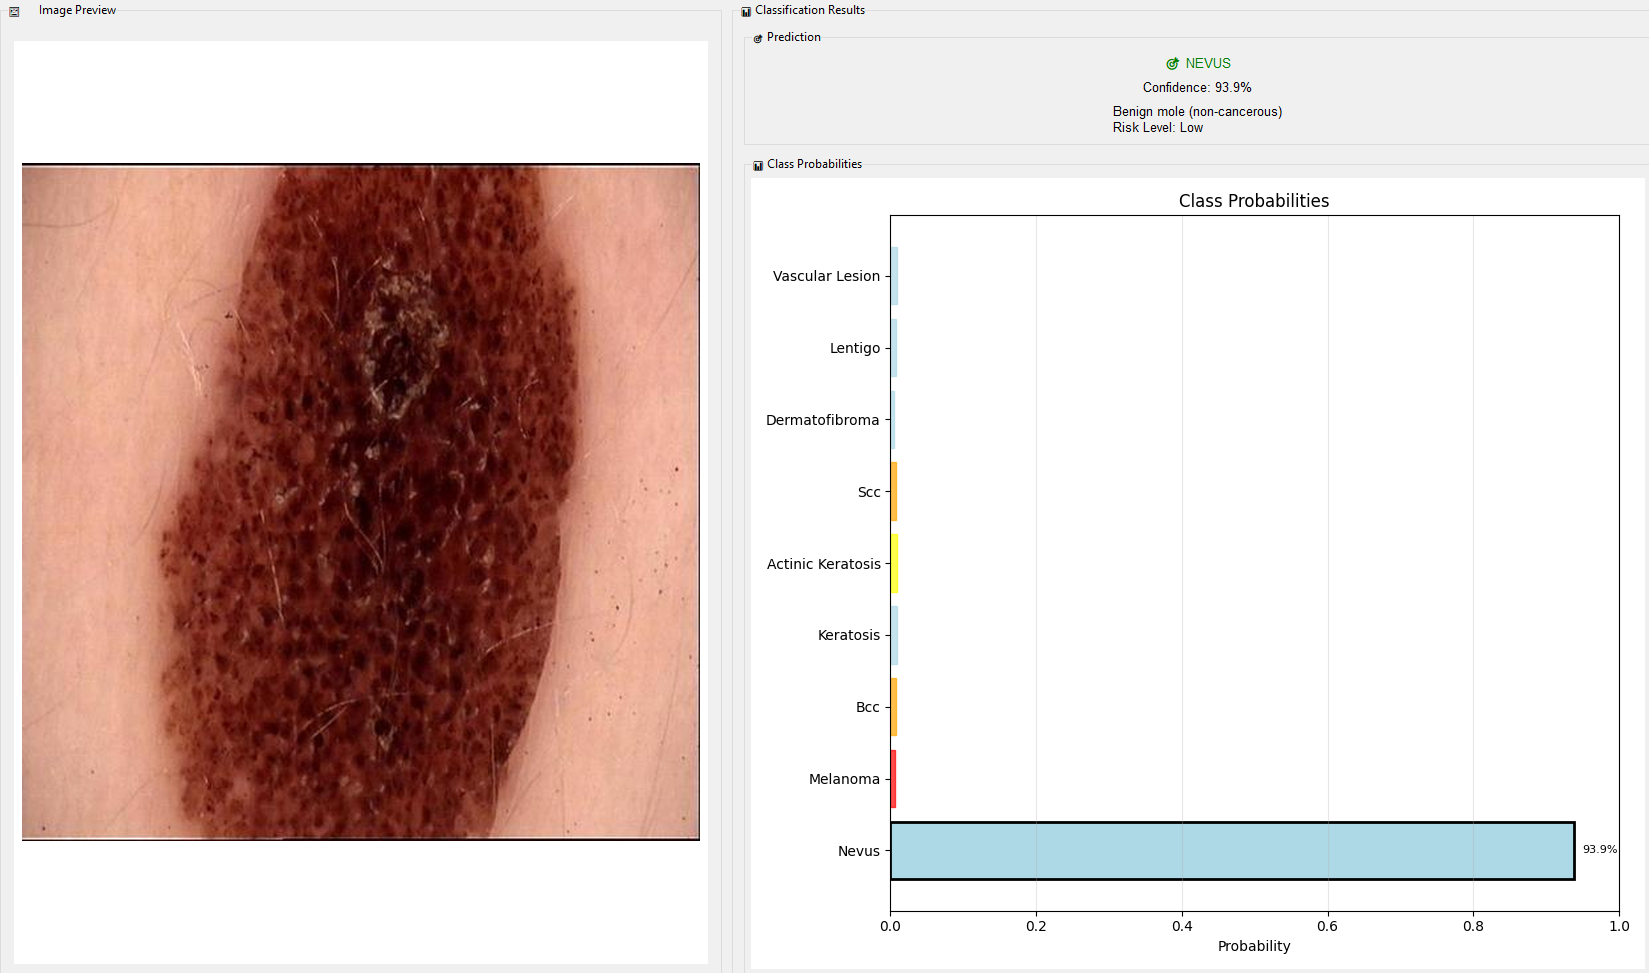
\includegraphics[width=0.6\textwidth]{Figs/nevus_prediction.png}
\end{center}
\caption{Model output on image with true label nevus, a majority class. The model correctly predicts nevus with 93.9\% confidence, demonstrating strong performance on well-represented classes.}
\label{fig:qual1}
\end{figure}

\begin{figure}[H]
\begin{center}
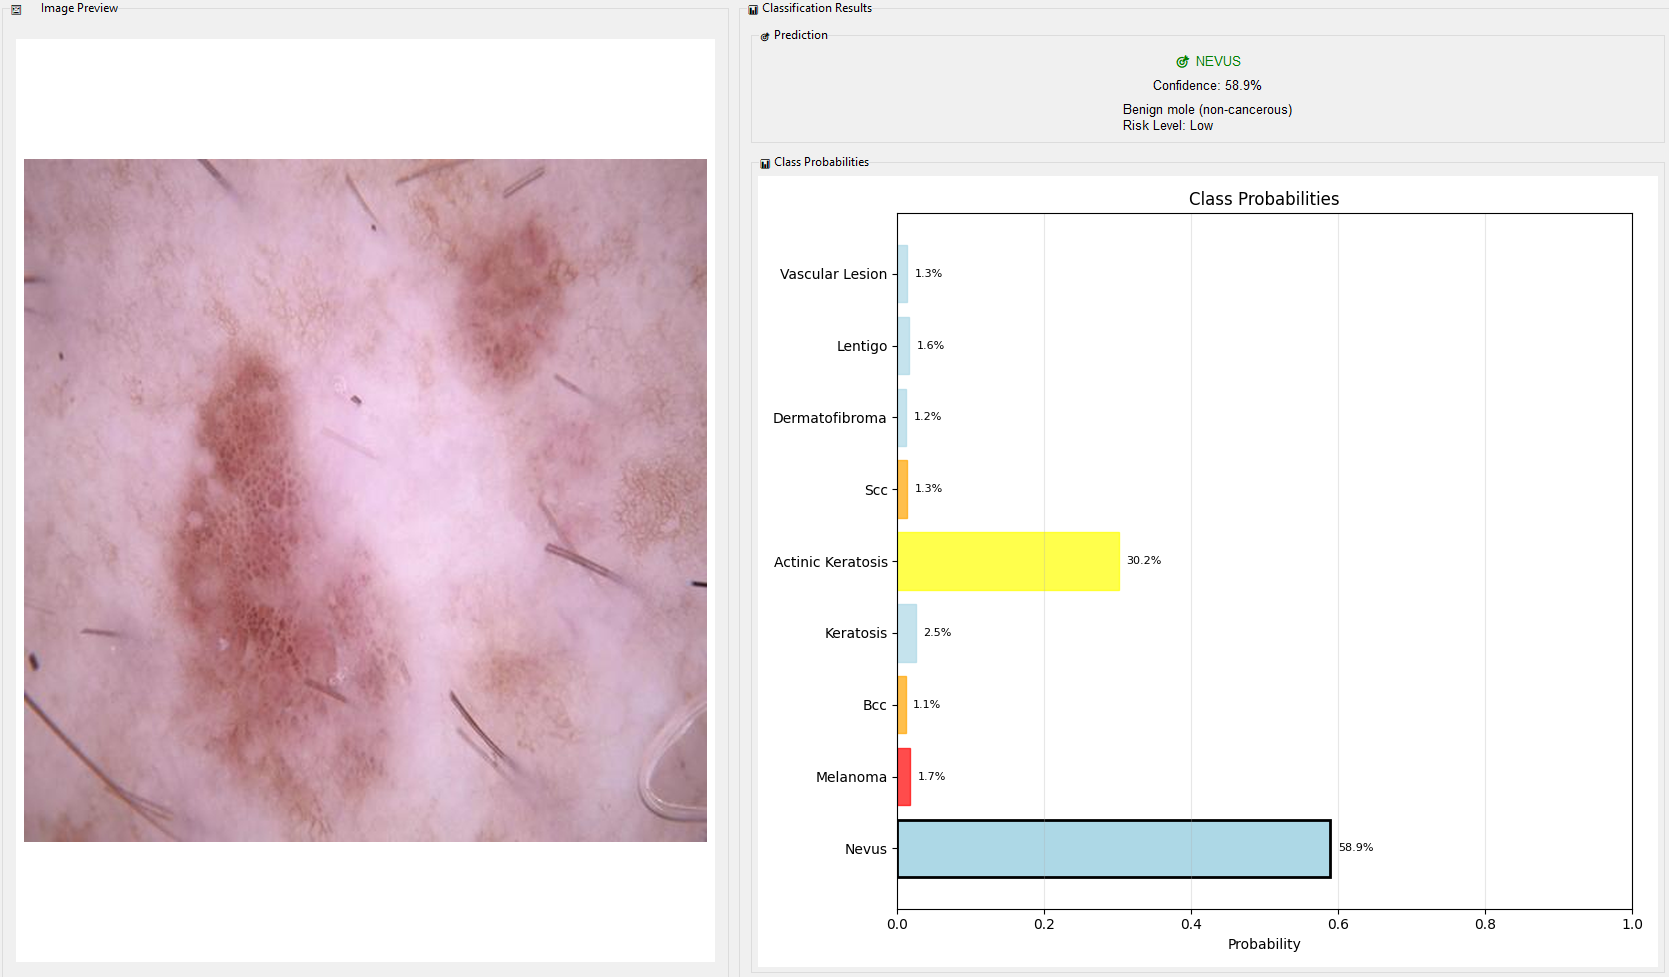
\includegraphics[width=0.6\textwidth]{Figs/actinic_prediction.png}
\end{center}
\caption{Model output on image with true label actinic keratosis, a minority class. The model incorrectly predicts nevus with 58.9\% confidence, reflecting uncertainty on rare conditions.}
\label{fig:qual2}
\end{figure}


We selected Figure~\ref{fig:qual1} and Figure~\ref{fig:qual2} to illustrate how class imbalance affects model performance. Figure~\ref{fig:qual1} shows strong performance on nevus (30.4\% of training data, 7,500 samples) with 93.9\% confidence, aligning with our 88.6\% precision results. Conversely, Figure~\ref{fig:qual2} shows lower confidence (58.9\%) and incorrect classification for actinic keratosis (only 1,473 samples), contributing to the 79.2\% recall for this class. The model appropriately exhibits uncertainty rather than overconfident predictions when training data is limited.

\section{Evaluation on Unseen Data}

The test dataset created in the data preprocessing stage was strictly separated from training and validation, ensuring unbiased evaluation of model generalization. No test images were used for hyperparameter tuning or architecture decisions. The model achieved 89.1\% accuracy, 91.3\% precision, 88.4\% recall, and 89.77\% macro F1 score on test data. These metrics are slightly lower than validation results, indicating minimal overfitting. Our regularization techniques successfully improved generalization, demonstrating that the model effectively distinguishes between nine skin conditions better than our baseline ResNet18-KNN approach (56.3\% accuracy).

\begin{table}[H]
\caption{Per Class Precision, Recall, and F1 scores.}
\label{per-class-results}
\begin{center}
\scriptsize
\begin{tabular}{|l|c|c|c|c|c|c|c|c|c|}
\hline
\textbf{Metric} & \textbf{nevus} & \textbf{melanoma} & \textbf{bcc} & \textbf{keratosis} & \textbf{actinic\_keratosis} & \textbf{scc} & \textbf{dermatofibroma} & \textbf{lentigo} & \textbf{vascular\_lesion} \\
\hline
Precision & 0.886 & 0.882 & 0.892 & 0.891 & 0.893 & 0.928 & 0.929 & 0.918 & 1.000 \\
\hline
Recall & 0.902 & 0.910 & 0.942 & 0.785 & 0.792 & 0.899 & 0.929 & 0.804 & 1.000 \\
\hline
F1 Score & 0.894 & 0.896 & 0.916 & 0.835 & 0.839 & 0.913 & 0.929 & 0.857 & 1.000 \\
\hline
\end{tabular}
\end{center}
\end{table}

\begin{figure}[H]
\begin{center}
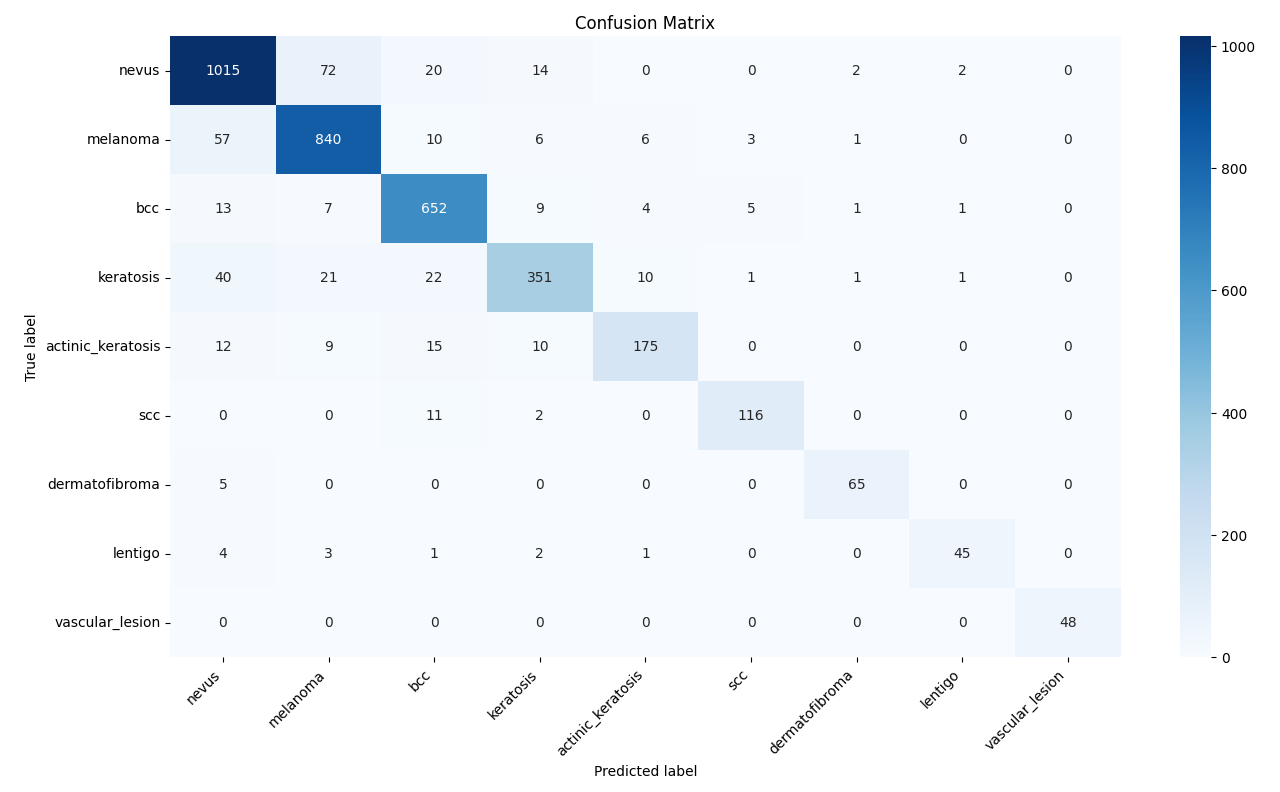
\includegraphics[width=0.8\textwidth]{Figs/test_confusion_matrix.png}
\end{center}
\caption{Confusion matrix of our best model checkpoint evaluated on our held out test data set.}
\end{figure}

\section{Discussion}

From a clinical perspective, our model's 89.1\% test accuracy represents a promising advancement in automated skin disease detection. This performance compares favorably to the reported accuracy of 74.1\% for dermatologists in similar classification tasks \citep{winkler2023assessment}. However, these comparisons must be interpreted carefully, as our model was evaluated on a specific set of nine skin conditions, whereas practicing dermatologists routinely diagnose hundreds of distinct dermatological conditions in clinical practice.

The model's ability to process both high-quality dermatoscopic images and smartphone-captured photos represents a significant advantage for patient accessibility. Many existing systems require specialized dermoscopy equipment, limiting their applicability in primary care settings or for patient self-screening. Our approach democratizes access to preliminary skin disease assessment, potentially enabling earlier detection and treatment initiation.

Despite achieving high overall accuracy, the model's performance varies considerably across different disease classes. The confusion matrix reveals that certain conditions, particularly those with lower representation in the training data, remain challenging to classify accurately. For instance, while the model achieves excellent performance on common conditions like nevus and melanoma, it struggles more with rare conditions such as vascular lesions and dermatofibroma. This performance disparity reflects the inherent challenge of learning from imbalanced datasets, even with the extensive class balancing techniques we employed.

The medical importance weighting system we implemented represents a novel contribution to the field. By assigning higher penalties to misclassifications of more clinically significant conditions (such as melanoma and squamous cell carcinoma), we aligned the model's learning objectives with clinical priorities. This approach resulted in improved detection rates for malignant conditions, though at the cost of slightly reduced overall accuracy for benign lesions.

Our data augmentation strategy, combining traditional geometric transformations with dermatology-specific techniques like CLAHE contrast enhancement, proved effective in improving model robustness. The use of Mixup and CutMix augmentation during training helped the model learn more generalizable features, as evidenced by the relatively small gap between validation and test performance. This suggests that our regularization techniques successfully prevented overfitting despite the model's large parameter count.

One significant limitation of our current approach is the absence of "healthy skin" samples in the training data. This forces the model to always predict a disease condition, which could lead to false positives when applied to images of normal skin in real-world scenarios. Future iterations should incorporate negative samples to improve the model's ability to distinguish between diseased and healthy tissue. Additionally, the dataset does not include any information about patient demographics or skin type, limiting our ability to assess potential biases in model performance across different populations.

\section{Ethical Considerations}

Our skin disease classification model raises important ethical considerations regarding healthcare AI deployment. Training datasets are inherently biased toward lighter skin tones, reflecting healthcare disparities and unequal documentation in darker-skinned populations \citep{alipour2024skin}. This bias could result in reduced model performance for patients with darker skin, potentially reinforcing existing healthcare inequalities. Additionally, false negatives in melanoma detection could delay critical treatment, while false positives may cause unnecessary patient anxiety. The model should serve as a diagnostic aid rather than a replacement for professional medical evaluation.

\section{Conclusion}

This project successfully developed a deep learning system for skin disease classification achieving 89.1\% accuracy on nine dermatological conditions. The Swin Transformer-based architecture, combined with comprehensive data augmentation and class balancing techniques, demonstrated significant improvements over the baseline ResNet18-KNN approach. The model shows promise as a preliminary screening tool, particularly for early detection of malignant conditions like melanoma.

Key contributions include the unification of four major dermatological datasets, implementation of medical importance weighting in the loss function, and achievement of performance levels comparable to dermatologists. However, limitations remain, including class imbalance effects on minority classes, absence of healthy skin samples, and potential dataset bias toward certain skin types.

Future work should focus on incorporating healthy skin data, improving minority class performance through advanced augmentation techniques, and validating the model on external datasets from different populations and imaging conditions. Additionally, developing uncertainty quantification methods could enhance clinical applicability by providing confidence measures for predictions.

\label{last_page}

\bibliographystyle{iclr2022_conference}
\bibliography{APS360_ref}

\end{document}
